\par{This implementation of this \emph{kernel} is as far as we know, the most 
    straightforward implementation of the matrix multiplication algorithm. 
    Optimisations were not implemented on this kernels as it can be seen in 
    listing \ref{naive_kernel}.} 
    
\par{Every instance of the \emph{kernel} calculates one element of the output 
    matrix(line 8), the \emph{NDRange} call is in 2 dimensions and all the 
    memory used for output and input data is global, this \emph{kernel}
    does not force caching or register usage via \emph{local} or \emph{private} 
    memory.}

\par{The results executing this kernel in different architectures with different 
    \emph{work group} dimensions can be seen in figure \ref{Naive}. From these 
    figures we can notice immediately that using dimensions greater than or 
    equal than 16 \emph{work items} in dimension 0 decreases the execution time 
    of the \emph{kernel} roughly 8 times in the case of Intel Xeon Phi. The
    Xeon CPU shows the same trend when the size of dimension 0 is greater or 
    equal than 2 but with an smaller decrease in execution time, 
    3.5 times approximately.}

\begin{figure}[!h]
    \centering
    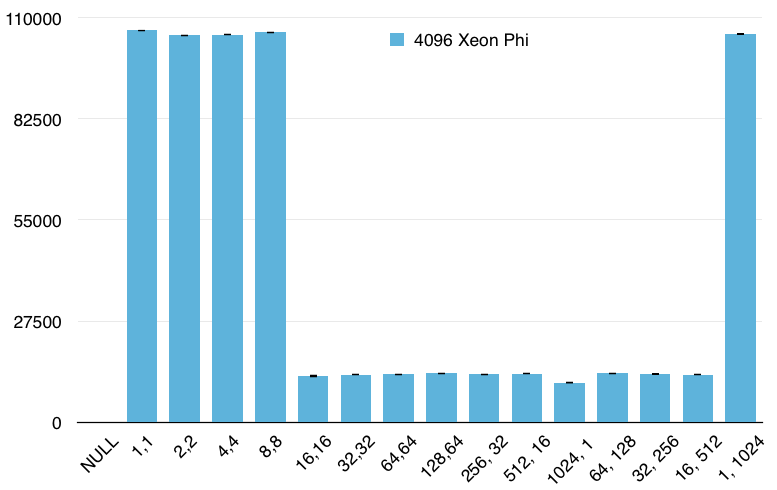
\includegraphics[width=0.49\textwidth]{figures/naive_phi.png}
    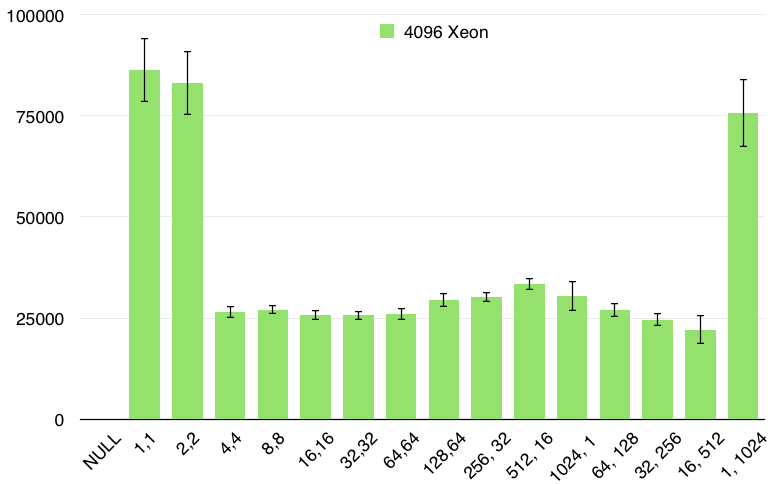
\includegraphics[width=0.49\textwidth]{figures/naive_cpu.png}
    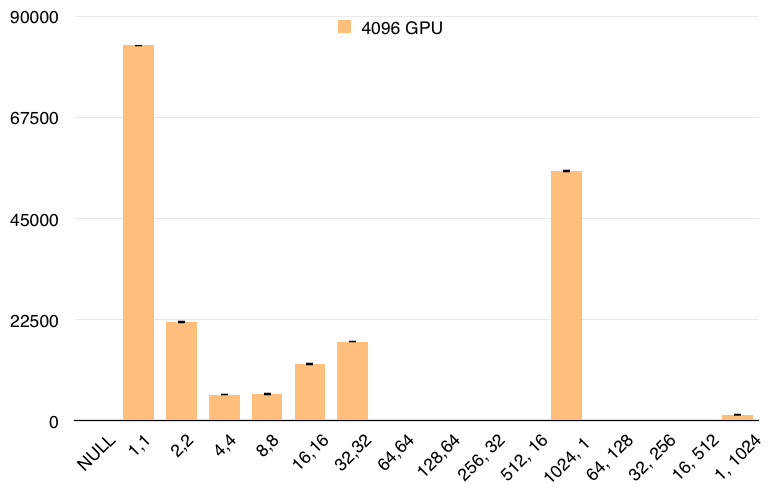
\includegraphics[width=0.49\textwidth]{figures/naive_gpu.png}
    \caption{Naive matrix multiplication results in different architectures.}
    \label{Naive}
\end{figure}

\par{Looking at listing \ref{llvm_code_naive_phi} we can realise that the 
    instructions that the Intel OpenCL compiler is generating are using a vector
    width of 16. This can explain the behaviour described previously and seen in
    figure \ref{Naive} for the Xeon Phi, being the \emph{work item} the basic 
    unit of computation in OpenCL, a \emph{work group} needs to have 16 \emph{
    work items} at least at dimension 0 to be able to use the entire width
    of the vector units available in the Xeon Phi. It seems that with numbers 
    less than 16 \emph{work items} inside of a \emph{work group} these 
    get serialized execution(using just one lane of the 16 available in the 
    vector registers of the Xeon Phi).}

\lstinputlisting[float,caption={Naive kernel LLVM code Intel Xeon Phi.}, 
    label={llvm_code_naive_phi}, 
    style=customc]
    {/Users/lalanne/MyCode/GitHubProjects/OpenCLNotes/src/code/llvm_naive_phi.ll}

\par{Listing \ref{llvm_code_naive_cpu} and figure \ref{Naive} show the same 
    behaviour in the Xeon CPU, but with vector width of 4 instead of 16. Thus 
    in this case the Xeon CPU only needs 4 \emph{work items} at dimension 0
    of a \emph{work group} for the vectorization start to work. One intesting
    thing to notice is that the Xeon CPU has hardware support for AVX 
    vectorization, this means that the vector width should be of 256 bits, 
    available to fit 8 single precision numbers. We can se that even though 
    the Xeon CPU has support for AVX still the Intel OpenCL compiler generates
    by default instruction using just half of the vector width available.}

\lstinputlisting[float,caption={Naive kernel LLVM code Xeon.}, 
    label={llvm_code_naive_cpu}, 
    style=customc]
    {/Users/lalanne/MyCode/GitHubProjects/OpenCLNotes/src/code/llvm_naive_cpu.ll}

\par{The way in which this \emph{kernel} is implemented, it shows poor data reuse
    forcing the system to request the data needed for computation from 
    \emph{global memory} using in a very inefficient way the cache system. 
    Figure \ref{vtune_naive} shows the profile of an execution of this \emph{
    kernel}, its possible to see the huge difference between the time that the
    \emph{kernel} spend bringing data from memory rather than using the data for
    computation(vgatherdps\footnote{Gather 2/4 packed 
    single-precision floating point values from memory referenced by the given 
    base address, dword indices and scale\cite{intrinsics}}
    \footnote{vgatherdps works by getting the data cache linewise per 
    invocation; this means that every time the gather instruction 
    is used, it will fetch only one cache line (CL), load all the values that 
    it is supposed to gather from it, store them in 
    the destination vector register, and finally zero out the bits of the 
    components that have been filled in the vector mask 
    register. As a consequence, the number of gather instruction depends on 
    the distribution of the data: 
    If all data resides in one CL then one gather instruction is sufficient; 
    in the worst case, each value is located in a different CL, 
    which will require sixteen gather instructions\cite{simd}.} vs vfmadd231ps).}

\begin{figure}[!h]
    \centering
    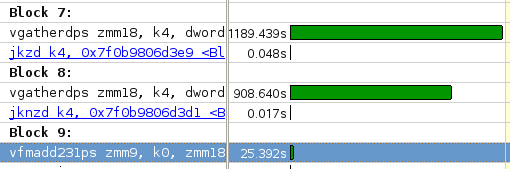
\includegraphics[width=0.49\textwidth]{figures/vtune_naive.png}
    \caption{Vtune profiler in the native kernel.}
    \label{vtune_naive}
\end{figure}

\par{{\color{red}Reading the listing \ref{naive_kernel}, its possible to see that there is no effort to use caches efficiently, the locality of
    memory access pattern its far from ideal. At the top of this, the gathering of data from memory results in having a high CPI(clock per
    instructions)\footnote{The CPI value of an application or function is an indication of how much latency affected its execution. 
    Higher CPI values mean there was more latency in your system – on average, it took more clockticks for an instruction to retire. 
    Latency in your system can be caused by cache misses, I/O, or other bottlenecks\cite{cpi}.} 
    rate poor vectorization and low L1 hit ratio for this kernel on the Xeon and Xeon Phi.}}

\par{For the GPU figure \ref{Naive} shows that not in all of the 
    \emph{work group} dimensions is possible to execute the kernel. 
    This is because the GPU run out of resources in those cases\cite{opencl_error},
    figure \ref{GpuDeviceInfo} and table \ref{tab:gpu_arch} show that the 
    maximum number of \emph{work group} size is of 1024 \emph{work items} which
    is exceeded by several of the \emph{work group} dimensions shown in figure 
    \ref{Naive}(\emph{e.g. 64x64}).}

\par{Figure \ref{NaiveRes} shows that GPUs achived the best performance in 
    comparison with the other architectures particularly
    in the case where the \emph{work group} dimension is 1x1024,
    this is mainly because the memory access patterns to access matrix A and B. 
    Access to matrix B its coalesced which means that the GPU can combine several 
    memory accesses into a single transaction, the memory access pattern for matrix 
    A also can be optimised, all the \emph{work items} in a warp access(read only)
    to the same memory space}.

\begin{figure}[!h]
    \centering
    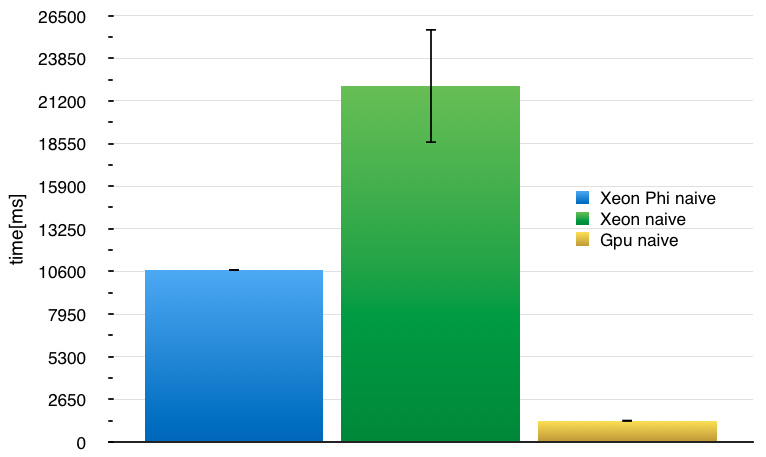
\includegraphics[width=0.49\textwidth]{figures/naiveRes.png}
    \caption{Comparison between the best cases in the different devices.}
    \label{NaiveRes}
\end{figure}

\par{Using warps and lock-step execution for the 
    GPU and vectorization of \emph{work items} for the Xeon and Xeon Phi, both
    memory access patterns are similar, with the difference that if we look at
    the GPU as a vector processor(warp execution) with double of the width that the
    Xeon Phi vector unit we can explain the better performance that this device 
    has against both Intel processors.}



